\clearpage
\newpage 
\section{Supplementary Materials for ReSumTool-30B}

\subsection{Cases of LLMs in Context Summarization}\label{appendix:summary_case}
\begin{figure}[!h]
    \centering
    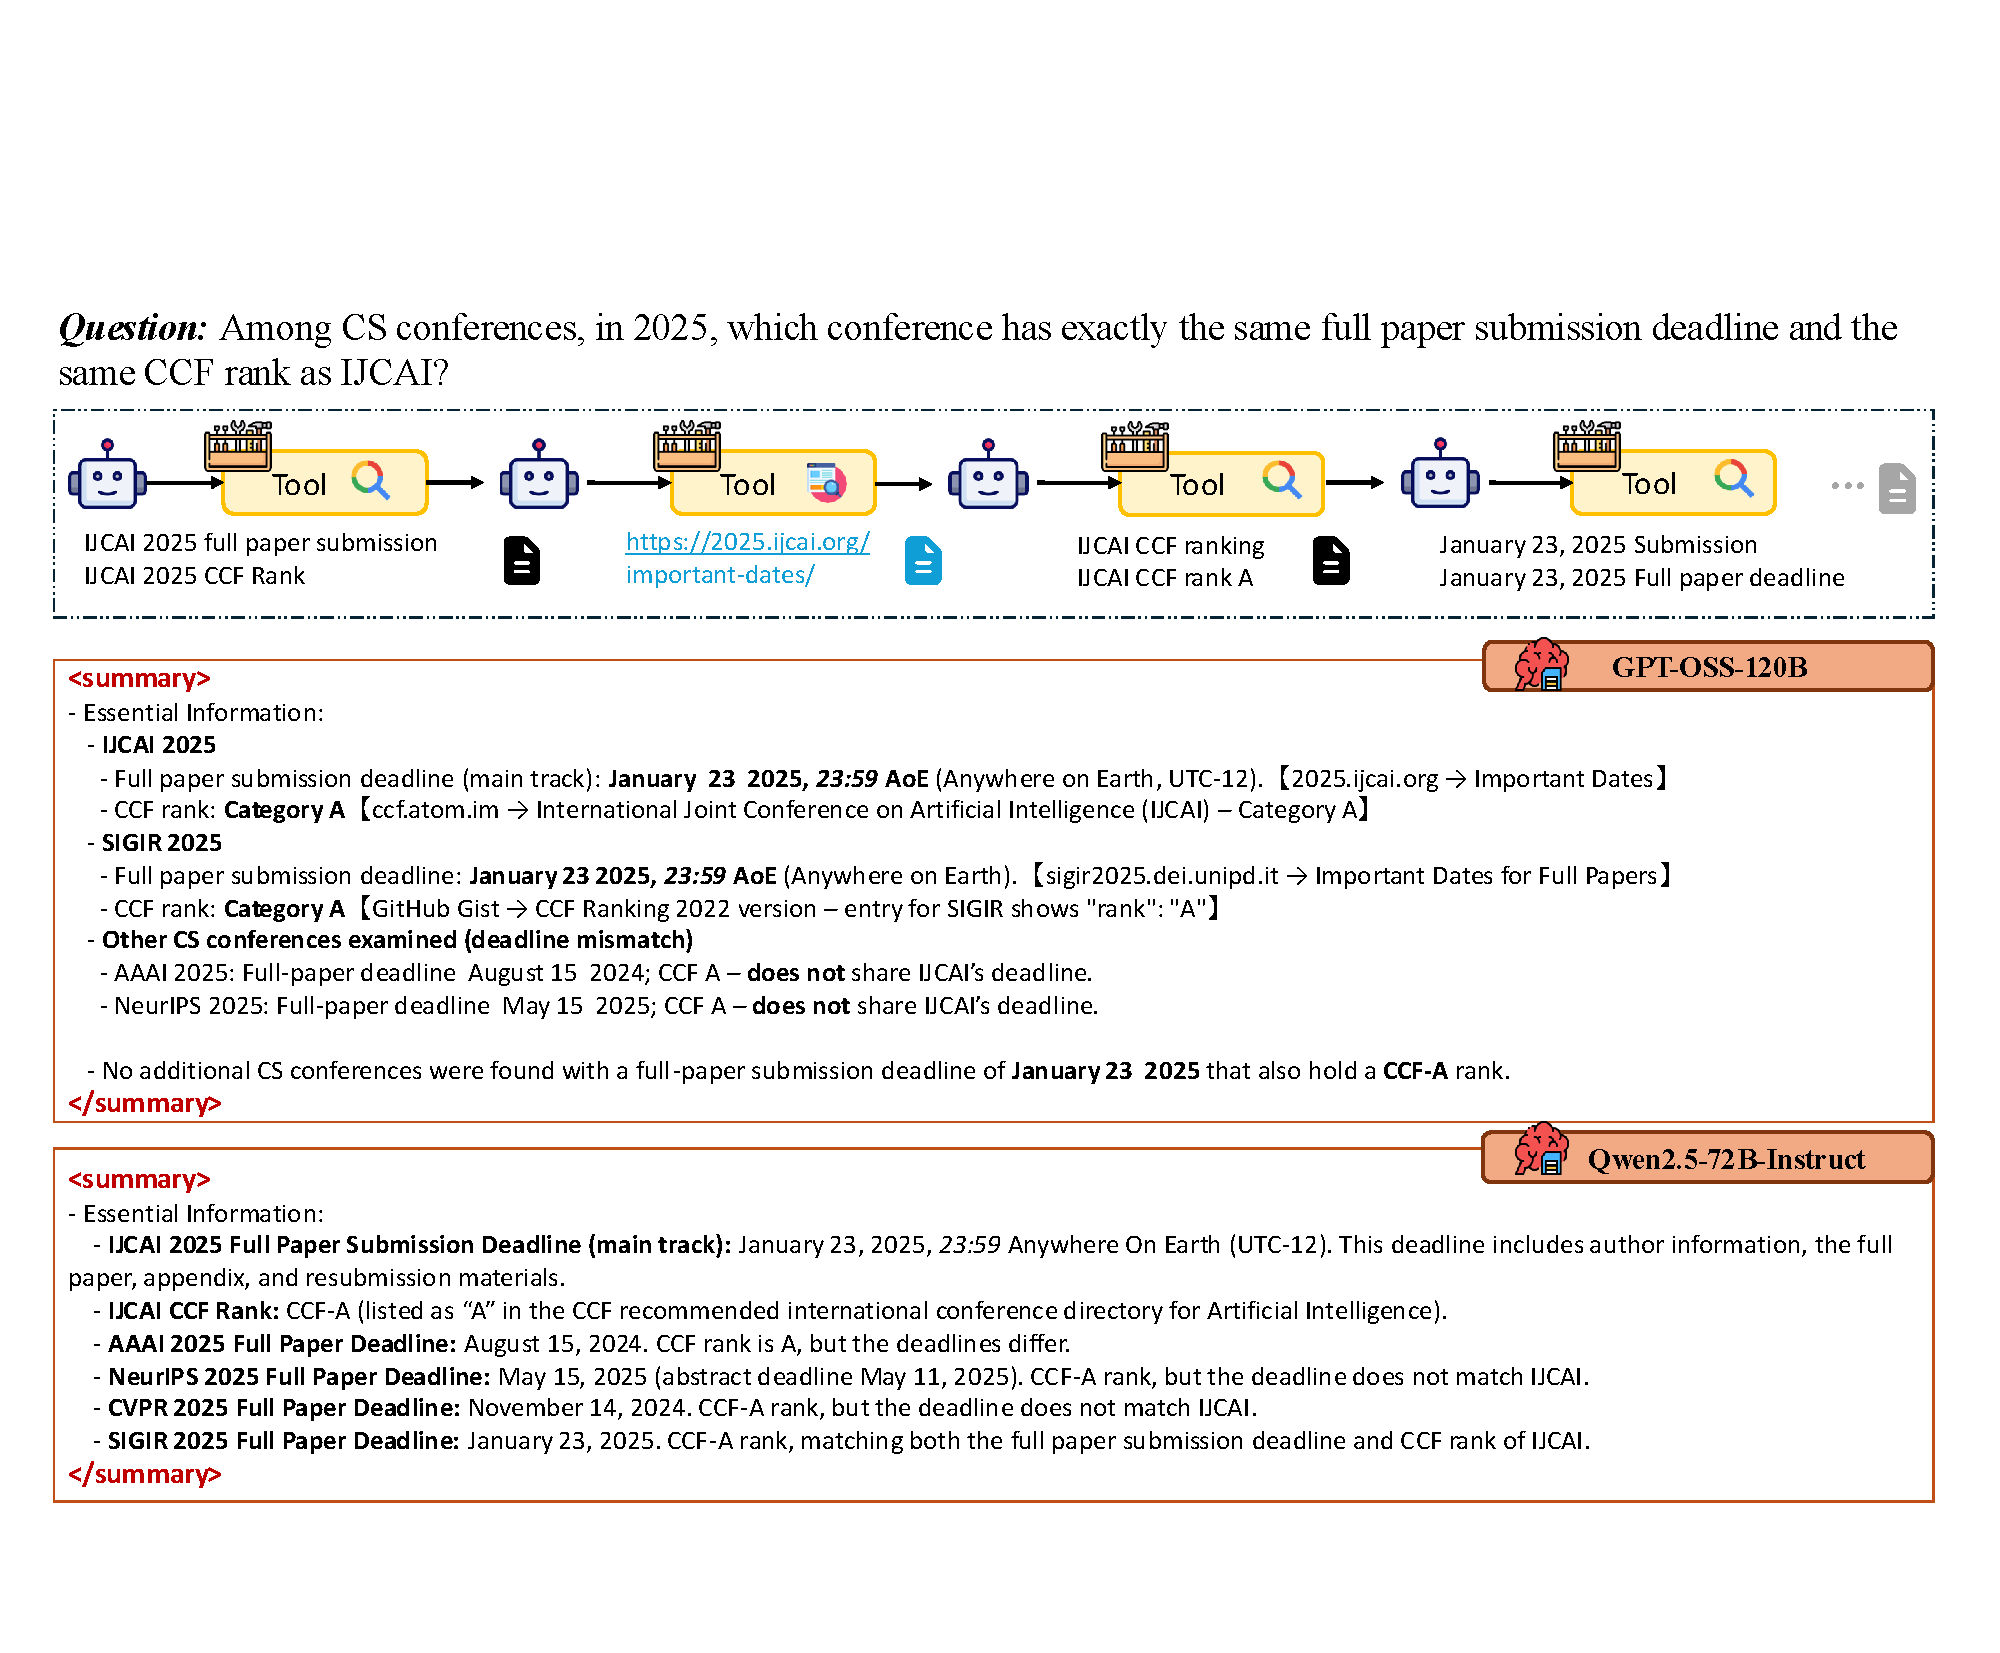
\includegraphics[width=\linewidth]{images/summary_comp.pdf}
    \caption{\textbf{Comparison between summary contents} generated by reasoning model GPT-OSS-120B~\citep{gpt-oss} and instruct model Qwen2.5-72B-Instruct~\citep{qwen2.5}.}
    \label{fig:summary_quality}
\end{figure}

We first conduct an empirical study comparing different models' context summarization capabilities, including a reasoning model GPT-OSS-120B and an instruction model Qwen2.5-72B-Instruct.

\textbf{Setting:} The target question is \emph{``Among CS conferences, in 2025, which conference has exactly the same full paper submission deadline and the same CCF rank as IJCAI?''}, with the ground truth answer being \textbf{\emph{SIGIR 2025}}. We let a web agent perform ReAct inference on this case and truncate the conversation to the first 10 rounds of interaction, where the agent actively searches for related conferences and has gathered some information that can lead to the ground-truth answer. We then use the prompt in Appendix \ref{appendix:prompt} to ask these two models to generate summaries, with output contents (highlighted parts aligned with the model's original output in Markdown format) shown in Figure \ref{fig:summary_quality}.

\textbf{Observation:} The comparison reveals significant differences in summarization quality and reasoning capabilities. GPT-OSS-120B demonstrates superior performance in several key aspects: (1) \textbf{structured organization} as it systematically categorizes information by conference with clear hierarchical formatting, (2) \textbf{comprehensive evidence gathering} as it identifies all relevant conferences and explicitly states why each candidate matches or fails the criteria, (3) \textbf{goal-oriented focus} as the summary directly addresses the question and highlights the final answer, and (4) \textbf{source attribution} as every piece of evidence is properly cited with specific sources. In contrast, Qwen2.5-72B-Instruct produces a more fragmented summary that lacks systematic organization. This  highlights the necessity for specialized reasoning capabilities in context summarization tasks, especially in complex web search scenarios where structured evidence synthesis is essential for agent guidance.


\subsection{Training Configurations}\label{appendix:resumtool_train}

In this subsection, we elaborate on the training process of ReSumTool-30B.

\textbf{Data Collection:} We collect $\langle \texttt{Conversation}, \texttt{Summary} \rangle$ pairs by performing ReSum rollout with WebSailor-30B as the agent and GPT-OSS-120B as the summary tool on a subset of the SailorFog-QA dataset~\cite{li2025websailor}. We select WebSailor-30B as the rollout model due to its zero API costs and satisfactory search intelligence compared to other open-source LLMs. The summary tool is fixed to GPT-OSS-120B due to its high-quality summary generation and open-source availability. The dataset is selected for its difficulty, as SailorFog-QA mirrors challenging benchmarks like BrowseComp, where agents must utilize summary tools to solve problems. The collected summaries undergo format checking and are combined with the query prompts, including conversation history, to form over \textbf{9K} $\langle \texttt{Input}, \texttt{Output} \rangle$ pairs. Here, \texttt{Input} represents the query prompt, while \texttt{Output} is the GPT-OSS-generated summary.
% 具体的数量:9345

\textbf{Training Hyper-parameters:} We use Qwen3-30B-A3B-Thinking~\citep{qwen3technicalreport} as the base model and perform supervised fine-tuning on the collected data. The training configuration includes a \texttt{batch\_size} of 64, 2 epochs, and a learning rate of $7 \times 10^{-6}$.


\subsection{Evaluation for ReSumTool-30B}
\begin{figure}[!h]
    \centering
    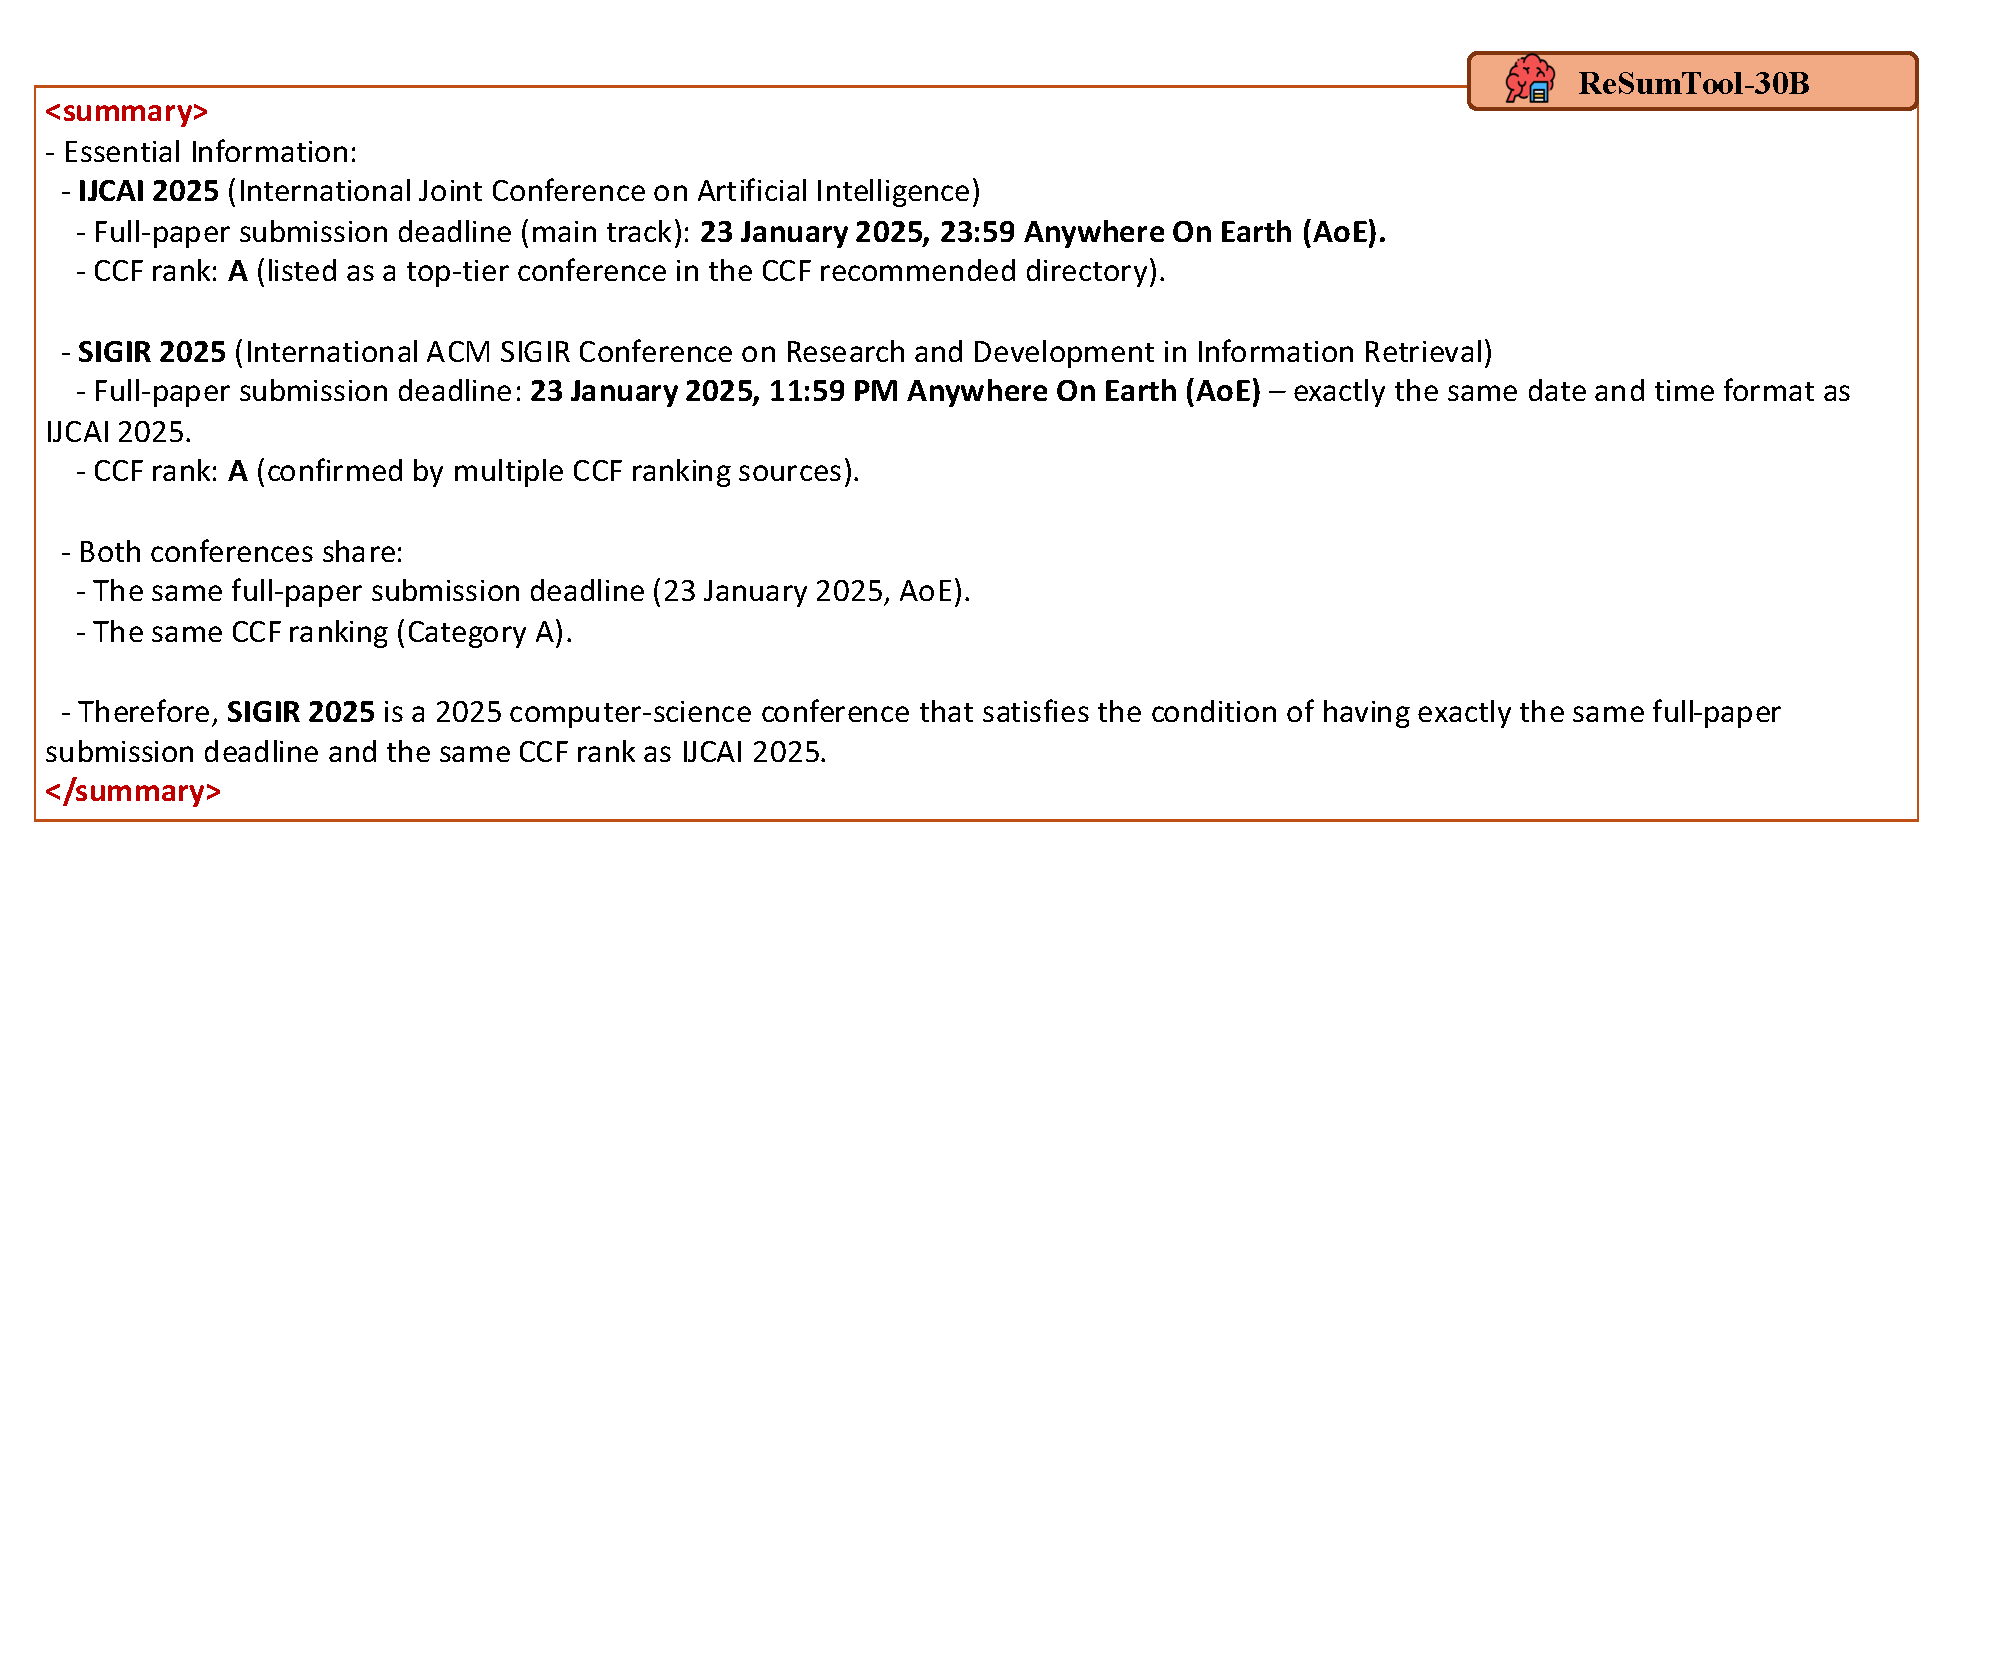
\includegraphics[width=0.96\linewidth]{images/summary_case2.pdf}
    \caption{\textbf{Illustration of summary content generated by ReSumTool-30B with conversation and question mentioned in Figure \ref{fig:summary_quality}}. The \textbf{highlighted} parts align with model's original output in Markdown format.}
    \label{fig:summary_case}
\end{figure}

To evaluate the performance of our trained model, we provide both quantitative results in Table \ref{tab:training_free_performance} and qualitative analysis in Figure \ref{fig:summary_case}.

\textbf{Quantitative Results:} We measure the summary capability through agent ReSum inference performance, as agents rely on summaries to resume exploration. As analyzed in the main text, by comparing results with larger large reasoning models like DeepSeek-R1-671B and larger instruction models like Qwen3-235B, integrating our ReSumTool provides \textbf{comparable} performance boosts and significantly outperforms the Qwen3-30B Base, demonstrating its effectiveness.

\textbf{Qualitative Analysis:} We further provide summaries generated by ReSumTool-30B for illustration in Figure~\ref{fig:summary_case}, where the solved question and conversation history exactly align with Figure \ref{fig:summary_quality}. From this case, we can see that summaries generated by ReSumTool-30B exhibit reasonable structures, goal-focused organization, and comprehensive evidence gathering.
